% vim:ts=4:sw=4
% Copyright (c) 2014 Casper Ti. Vector
% Public domain.

\chapter{高速公路社群划分方法}

	上一章介绍了面向高速公路的关键节点挖掘模型,并给出了贪心算法。然而根据模型的定义,就算进行简化,认为关键路段已经选出,计算对关键路段进行维护之后的整体网络通行效率也需要$2^n$的时间复杂度。虽然说高速公路上只有部分路段出现过损毁情况,n的规模比较小,勉强可以求解,但是当高速公路网络扩大时,指数级别的复杂度不可接受。

	\section{模型分析}
		模型需要从输入的代表关键节点的离散0-1向量$\bm{y}$,求得高速公路网络通行效率的期望。对于这种输入为整数或整数向量,并且内部具有概率事件的问题,本质上属于随机整数规划问题。在数学优化领域,随机规划是一个涉及不确定性优化问题的框架。比如说两阶段线性规划。决策者在第一阶段采取一些行动,之后发生随机事件影响第一阶段决策的结果。不断调整第一阶段的决策,使得整体期望收益达到最大。

		现有的随机整数规划问题大都是基于班德斯分解方法(Benders Decomposition)进行研究,然而班德斯优化方法要求有两层模型,且两层模型之间互不影响。本研究中,第一层的决策变量$\bm{y}$会直接影响到第二层里面的路网拓扑结构概率,对于这种相互依赖的随机规划问题,现有的研究并没有一些比较合适的优化方法。

	\section{高速公路社群划分模型}

		%查重
		\subsection{模型定义}
			复杂网络具有社群特性,高速公路属于复杂网络的一种。给定高速公路有向图$G=\{V,E\}$,其中V代表收费站(节点)的集合;E表示边的集合。定义社群$c=\{v_1,v_2,...v_m\}$,其中$v_i$是网络中的节点,即收费站或者交叉路口;社群集合$C=\{c_1,c_2,...c_u\}$;其中$v_i \in V$,${c_i}\bigcap {{c_j}}  = \emptyset$,$\sum\limits_{i = 1}^u {\sum\limits_{v \in {c_i}} v  = V}$。

			基于高速公路社群划分的关键节点挖掘算法主要采用分治思想,将一个难以直接解决的大问题,分割成一些规模较小的相同问题,以便各个击破,分而治之。本文主要将路网分成一个个子路网,在子路网中分别计算关键节点,之后再用一定的方法合并。在此需要解决两个问题:

				1)如何分群

				2)分群求解后,如何合并

			传统的复杂网络社群划分系统中,大都是针对虚拟网络(如社交网络)进行研究。高速公路网络和虚拟网络有很大的不同。在虚拟网络中,两个点之间只要有交流,那就代表有边相连;在高速公路中,我们认为只要两个收费站有流量交流,即O-D不为0,那么这两个收费站之间就有边连接(不同于上一章的路网定义)。但是这个边和其他的复杂网络如社交网络不同,社交网络中两个节点之间的空间距离就是1跳,但是对于物理网络来说,两个节点之间的边具有实体距离。高速公路中路段之间的影响也会根据物理距离的变化而变化,这些都是传统方法中没有考虑到的。

			2004年,Newman和Girvan[]提出了一个用于刻画网络社区结构优劣的量化标准,被称作模块化函数。简单的带权模块化函数定义如下:

			\begin{equation}
			Q = \frac{1}{{2m}}\sum\limits_{ij} {[{A_{ij}} - \frac{{{k_i}{k_j}}}{{2m}}]\delta ({c_i},{c_j})}
			\label{eq4}
			\end{equation}

			式\ref{eq4}中,$A_{ij}$表示节点$i$和节点$j$之间的边权;$k_i=\sum\limits_{j} {A_{ij}}$表示所有与节点i相连的边的边权和;$c_i$是指i所属的社群编号;如果$c_i=c_j$,那么$\delta (u,v)=1$,否则等于0;$m=\frac{1}{{2}}\sum\limits_{ij} {A_{ij}}$。

			模块化函数主要用于度量社群划分结构的优劣,现有的基于模块化函数的分群算法都没有考虑高速公路的特性\parencite{},并且在高速公路网络上出现了低分辨率特性和极端退化特性\parencite{}。Newman提出了一种社群挖掘方法\parencite{}:初始的时候没个节点都是一个社群,之后进行迭代,每次迭代时都选择使目标模块函数在Q增加最大的社群进行合并。这个方法虽然在时间效率上很高,但是没有解社群划分的决极端退化特性。Guimera提出一种基于模拟退火的模块性优化方法:初始解是随机生成的社团集合,在每次迭代过程中,采用一定策略,结合当前解生成新的解集,用模块化函数Q判断解集的优劣,最后用模拟退火中的Metropolis准则来决定是否采用该解。这个方法虽然在一定程度上解决了极端退化特性,但是他有一个很严重的问题,在相通的输入集合上,生成的最终结果往往不同,不符合稳定性要求,而且时间复杂度大,求解效率低。Blondel\parencite{}提出快速模块优化方法,他认为首先在局部使用局部模块化函数f获得局部社团,然后再对这些局部社团作为一种超级节点,再进行合并,不断迭代,直到模块化函数Q不再增加为止。这个聚类方法存在聚类社团过大的情况,不符合本文中缩小节点量级,优化算法时间复杂度的目的。针对现有研究的不足,结合高速公路的路网特性,在此提出面向高速公路的社群划分模块化函数Q:

			\begin{equation}
			\vartriangle Q = [\frac{{\sum_{in} C  + 2{k_{i,in}}}}{{2m}} - {(\frac{{\sum_{tot} C  + {k_i}}}{{2m}})^2}] - [\frac{{\sum_{in} C }}{{2m}} - {(\frac{{\sum_{tot} C }}{{2m}})^2} - {(\frac{{{k_i}}}{{2m}})^2}] - L(i)
			\label{eq5}
			\end{equation}

			公式\ref{eq5}用于在遍历过程中,判断节点应该属于哪一个社群。式中,$\sum_{in} C$表示社群$C$内部的所有边的权重和;$\sum_{tot} C$表示所有与社群$C$中的节点相连的边的权重和;$k_{i,in}$表示$i$到$C$中所有节点之间的连线的权重和;$k_i$表示所有和节点i直接相连的边的权重和;m是路网中所有边的权重之和;$L(i)$是模型罚项,代表i转移社群后,不同社区之间交通流的变化。

			$L(i)$:

			\begin{equation}
			L(i)=\frac{{{k_{i,{c_1}}} - {k_{i,{c_2}}}}}{{{k_{{c_1},{c_2}}}}}
			\label{eq6}
			\end{equation}

			式\ref{eq6}中,${k_{i,{c_1}}}$表示路段i流向社群$c_1$的流量,$k_{i,{c_2}}$代表路段i流向社群$c_2$的流量,${{{k_{{c_1},{c_2}}}}}$表示社群$c_1$,$c_2$中所有节点之间的流量和。

			在本节模型中,边的权重不止与两个节点之间的流量有关,还与两个节点之间的物理距离有关。和传统复杂网络不同,节点之间的距离不再由节点之间的最短跳数决定,而是由节点之间的最短物理距离$L$决定。$L_{ij}=\sum\limits_{e \in E_{ij}} {e}$,式中$E_{ij}$是节点i和节点j之间的最短路径中路段的集合。定义边权重$W_{ij}=\frac{f_{ij}}{L_{ij}*T}$。由于社群划分算法具有极端退化特性,



		\subsection{模型分析}
			高速公路网络除具有绝大多数复杂网络的特征外,作为空间网络还具有不同于抽象网络的特性,这些特性决定了高速公路网络的拓扑性质。具体可以归纳为:高速公路交通网络的节点存在于二维地理空间,且有明确的位置;高速公路网络中的边是一种实体联接,具有明确意义,并不是抽象空间中所定义的关系,能够明确表示线路之间的相互关系,线路在整个网络中的重要程度以及网络的局部和全局效率;高速公路交通网络中节点的长程联接需要一定成本,这一特性直接影响着高速公路网络出现小世界行为的可能性;高速公路交通网络中单一节点所能联接的边的数目受到物理空间的限制,这种限制会影响到网络的度分布。

			在以前的高速公路项目研究中,我们发现低跳数的用户占大多数。如图$\ref{fig4}$,可以发现在高速公路中,低跳数的车辆占了大多数,10跳以下的车辆占所有车辆总数的90\%以上。再结合高速公路的异质性,复杂网络的社群性,我们认为高速公路网络应该也具备社群性质,即存在一个个社群,这些社群各自包含一些收费站和高速公路路段,高速公路中的车辆大都从社区内部的节点出发,在同一个社区的另一个节点驶离。社区之间的车辆交流尽量小。

			\begin{figure}[h]
			\centering
					\begin{minipage}{0.8\linewidth}
						\centering
						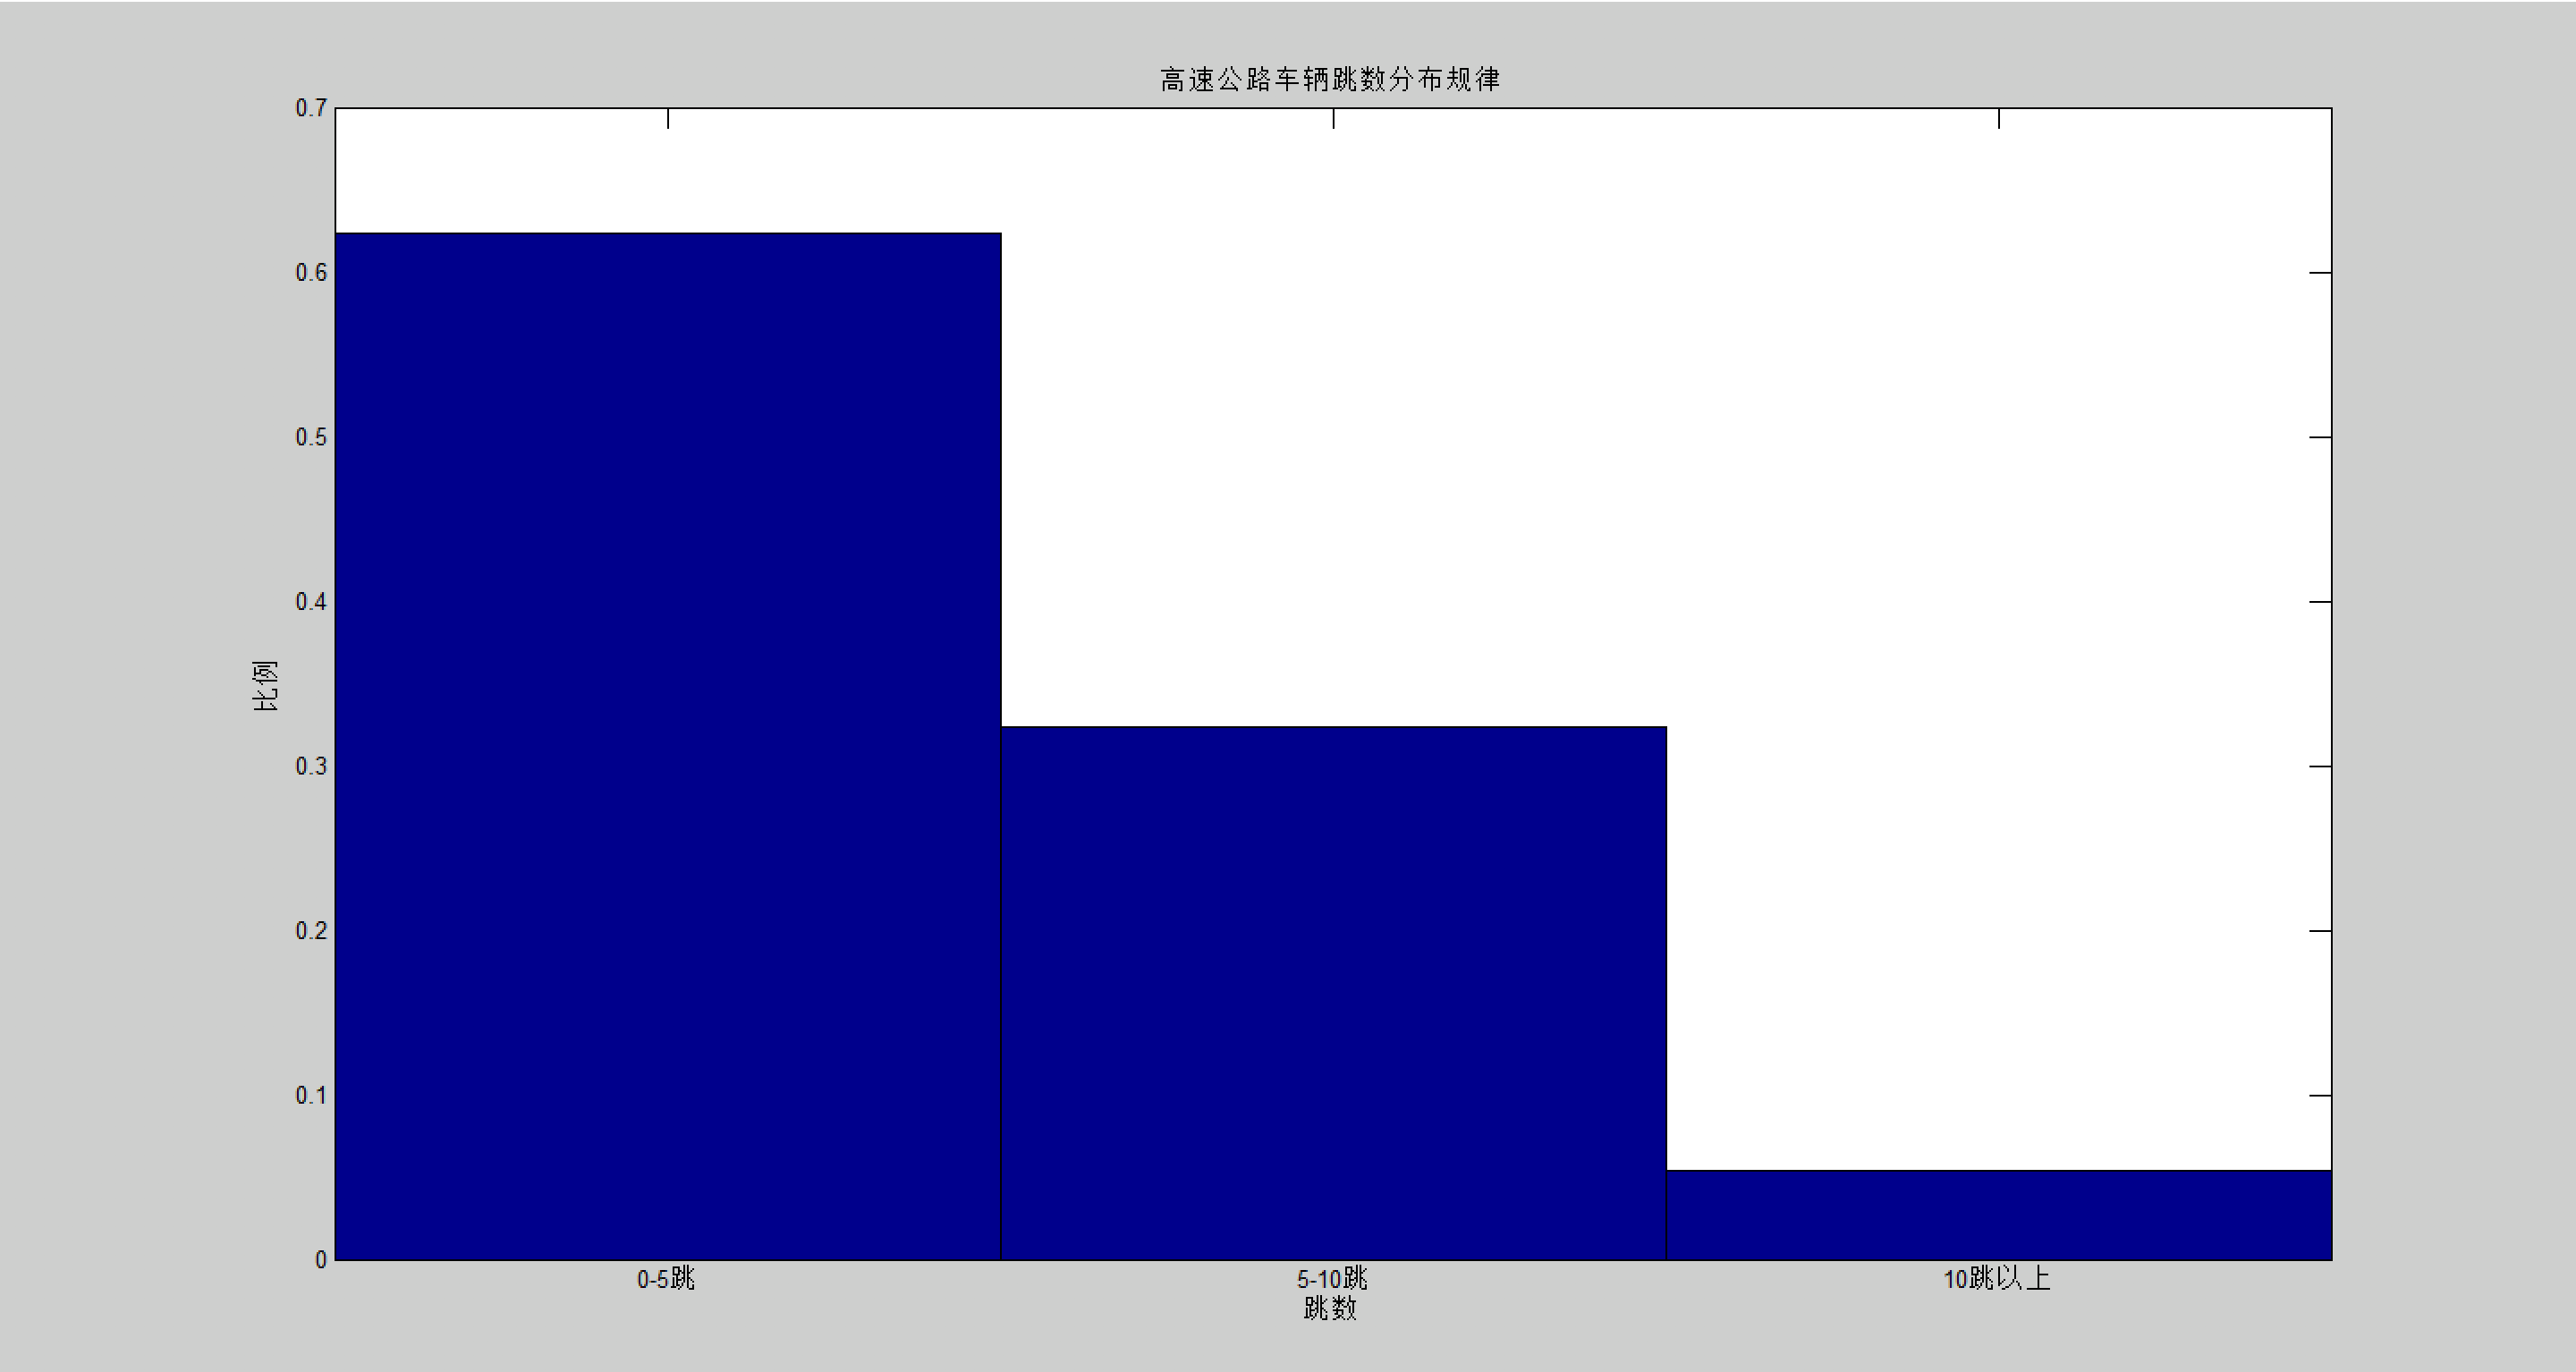
\includegraphics[width=4.4in]{picture/tiaoshu}
						\caption[这是一个有味道的图]{fig1}
						\label{fig4}
					\end{minipage}%\
			\end{figure}

			为此,抽取某一天的高速公路O-D数据,将有O-D交流的收费站之间连线,流量越多,线的颜色越深,流量越少,线的颜色越浅。如图\ref{fig5},可以较直观的看出高速公路的社群特性。

			\begin{figure}[h]
			\centering
					\begin{minipage}{0.8\linewidth}
						\centering
						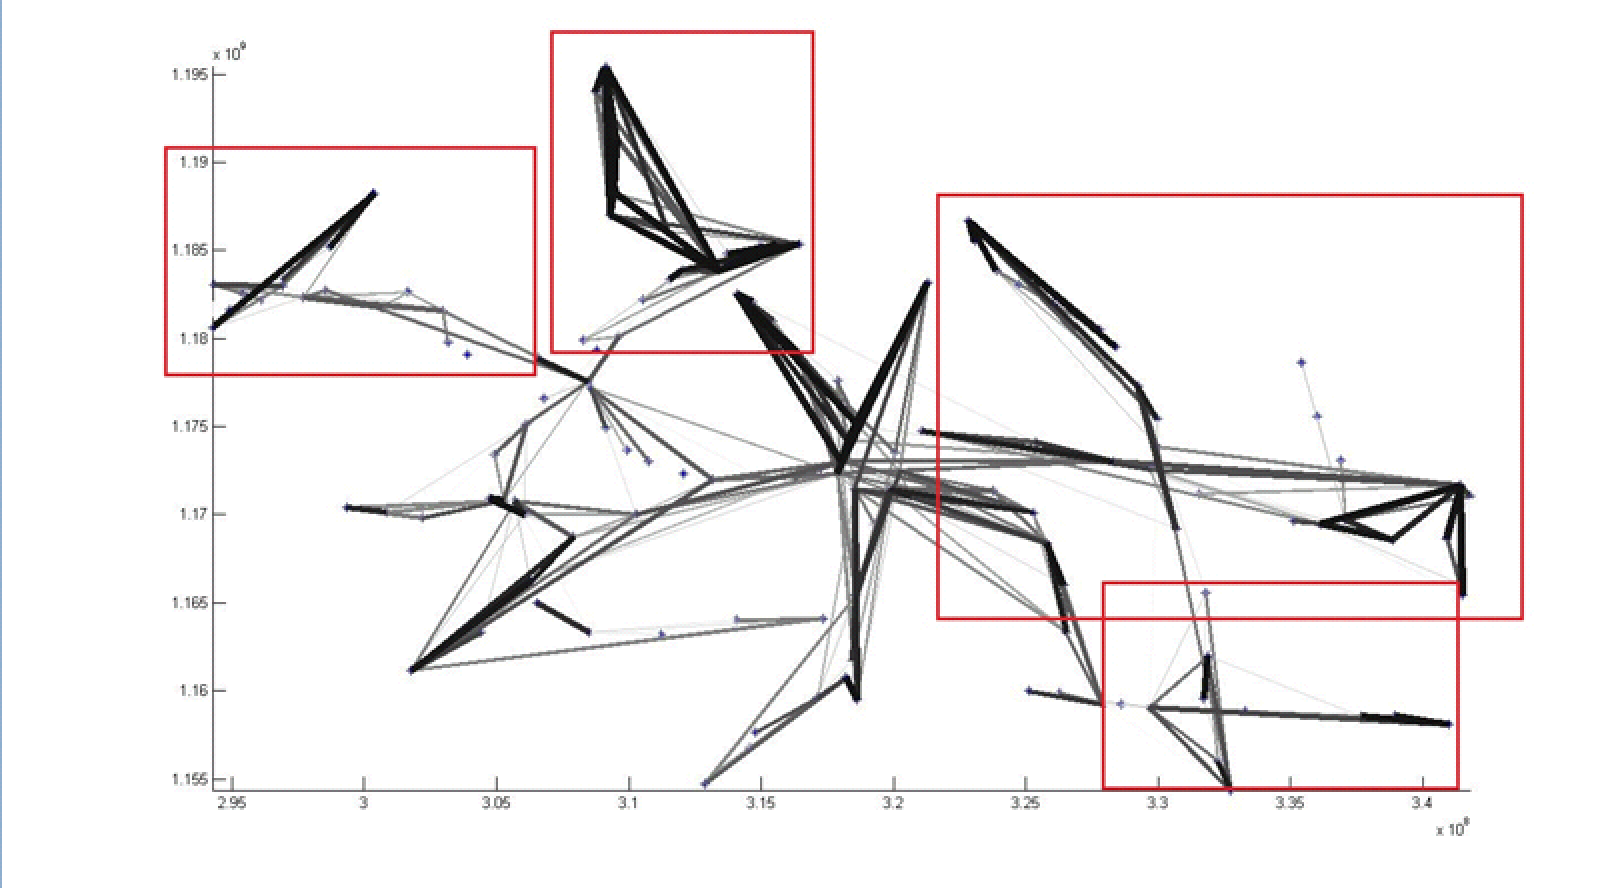
\includegraphics[width=4.4in]{picture/shequntexing}
						\caption{fig1}
						\label{fig5}
					\end{minipage}%\
			\end{figure}
		\subsection{模型实现}
			高速公路社群划分的目的是将整个高速公路拓扑结构分成一个个社区,使得社区内部交流尽量多,社区之间的交流尽量少,最终在各自社群分别计算关键节点,分治计算,最后进行合并,达到优化时间复杂度的目的。在此引入基于模块性优化的社区挖掘方法。

			2004年,Newman和Girvan[]提出了一个用于刻画网络社区结构优劣的量化标准,被称作模块化函数。简单的带权模块化函数定义如下:

			\begin{equation}
			Q = \frac{1}{{2m}}\sum\limits_{ij} {[{A_{ij}} - \frac{{{k_i}{k_j}}}{{2m}}]\delta ({c_i},{c_j})}
			\label{eq4}
			\end{equation}

			式\ref{eq4}中,$A_{ij}$表示节点$i$和节点$j$之间的边权;$k_i=\sum\limits_{j} {A_{ij}}$表示所有与节点i相连的边的边权和;$c_i$是指i所属的社群编号;如果$c_i=c_j$,那么$\delta (u,v)=1$,否则等于0;$m=\frac{1}{{2}}\sum\limits_{ij} {A_{ij}}$。

			基本的社群划分存在分辨率限制和极端退化特性。分辨率限制是指社群划分方法无法发现小于一定规模的社群,极端退化特性是指最终的社群划分结果会收敛于指数数量级的高分解决方案,而不是指向一个或少量最优解。[xxx]采用一种方法解决低分辨率问题:初始化时,将每一个节点看作一个独立的社群,之后根据模块化函数不断循环修正节点的所属社群。这个方法用在高速公路上时,虽然解决了低分辨率社群无法发现的问题,但是最终会产生一系列孤立点(如图\ref{gulidian}),这不符合社群划分的初衷。而且最终结果也没有避开极端退化特性,最终的社群划分结果在一个非常大的解空间中循环。

			\begin{figure}[h]
			\centering
					\begin{minipage}{0.8\linewidth}
						\centering
						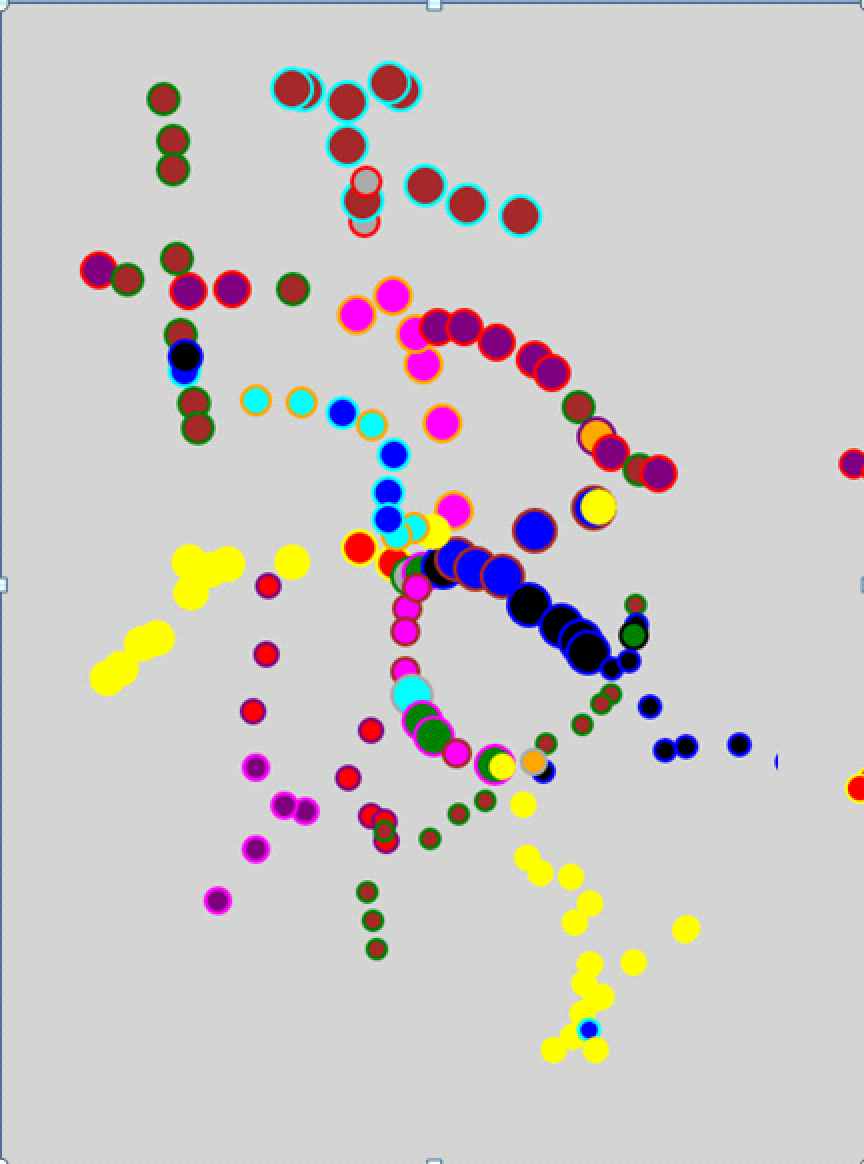
\includegraphics[width=4.4in]{picture/liuliangbianquan}
						\caption{fig1}
						\label{gulidian}
					\end{minipage}
			\end{figure}

			在此,结合高速公路路网特性以及本文的研究目标,作出以下几项改进:

			1)在边权中引入路段物理长度:高速公路网络是具有实体的物理网络。为了找到符合本文要求的社区,我们认为只要两个收费站有O-D交流,那么这两个收费站之间就有边连接(不同于上一章的路网定义)。但是这个边和其他的复杂网络如社交网络不同,社交网络中两个节点之间的距离就是1跳或者其他权值,但是对于物理网络,它具有实体距离。在此定义两个收费站i,j之间的距离,令$e={e_1,e_2...e_n}$表示i和j之间的最短路径中的路段集合,本文认为i和j的距离$D=\sum {len(e_k)}$。这个方法可以解决一部分孤立点和交叉社区

			2)采用模拟退火思想,不断变化边权——增加距离的权重,直到解集收敛,或者新的解集的规模变化大于退火温度:这个方法主要用于使解集收敛,解决极端退化特性。

			社群划分基准函数:
			\begin{equation}
			\vartriangle Q = [\frac{{\sum_{in} C  + 2{k_{i,in}}}}{{2m}} - {(\frac{{\sum_{tot} C  + {k_i}}}{{2m}})^2}] - [\frac{{\sum_{in} C }}{{2m}} - {(\frac{{\sum_{tot} C }}{{2m}})^2} - {(\frac{{{k_i}}}{{2m}})^2}] - L(i)
			\label{eq5}
			\end{equation}

			公式\ref{eq5}用于在遍历过程中,判断节点应该属于哪一个社群。式中,$\sum_{in} C$表示社群$C$内部的所有边的权重和;$\sum_{tot} C$表示所有与社群$C$中的节点相连的边的权重和;$k_{i,in}$表示$i$到$C$中所有节点之间的连线的权重和;$k_i$表示所有和节点i直接相连的边的权重和;m是路网中所有边的权重之和;$L(i)$是模型罚项,代表i转移社群后,不同社区之间交通流的变化。

			$L(i)$:

			\begin{equation}
			L(i)=\frac{{{k_{i,{c_1}}} - {k_{i,{c_2}}}}}{{{k_{{c_1},{c_2}}}}}
			\label{eq6}
			\end{equation}

			式\ref{eq6}中,${k_{i,{c_1}}}$表示路段i流向社群$c_1$的流量,$k_{i,{c_2}}$代表路段i流向社群$c_2$的流量,${{{k_{{c_1},{c_2}}}}}$表示社群$c_1$,$c_2$中所有节点之间的流量和。下面说明算法步骤。

			初始权重设为$f/l$,$f$表示两个节点之间的流量,$l=\sum {len(e)}$表示两个节点之间的物理距离。$e$表示两个节点之间的最短路径。初始情况下,每个节点都构成一个社群,对节点进行遍历,运用公式\ref{eq5},判断节点应该属于哪一个社群。循环到节点社群无变化或者社群分类进入循环的状态,停止本次迭代,改变权值,进行下一轮迭代,直到收敛。

			伪代码如下:
			\begin{algorithm}[h]
	        \caption{高速公路社群划分方法}  
	        \label{shequn}
	        \begin{algorithmic}[1] %每行显示行号  
	            \Require 高速车辆O-D数据,高速公路网络拓扑结构,最大社群节点数量
	            \Ensure 高速公路社群划分结果
	            \Function{Community}{$ODMatrix,G={V, E},B$}  
	                \State $res\gets [[\{0,0\},\{1,1\},\cdots,\{n,n\}]]$ 
	                \State $tmp\gets [\{\}]$
	                \State $pre\gets [[\{0,0\},\{1,1\},\cdots,\{n,n\}]]$ 
	                \State $k\gets 0$  
	                \State $l\gets 0$
	                \State $T\gets 100$  
	                \While{$|len(res)-len(pre)| \leqslant T$}
	                	\State $res=res[-1]$
	                	\State $pre=res$
	                	\While{$res[-1] \not\subset res[0:-1]$}
		                	\State $tmp\gets res[-1]$  
		                	\For{$i \in E $}  
		                		\For($C \in tmp \& |C| \le B$)
		                			\If{$\vartriangle Q > k$}  
			                        	\State $l\gets C$  
			                        	\State $k\gets {\vartriangle Q}$  
		                    		\EndIf	
		                		\EndFor
		                    	\State $tmp[l] \gets i$ 
		                	\EndFor
		                	\State $res \ add \ tmp$
	                	\EndWhile
	                	\State T--
	                \EndWhile  
	                \State \Return{$res$}  
	            \EndFunction  
	        \end{algorithmic}  
	    	\end{algorithm} 

			采取自下而上的策略,可以有效解决低分辨率问题;而基于高速公路的物理网络特性,对边权值进行处理,可以增加算法结果的收敛程度;最后用模拟退火思想,逐渐加强距离的权重,达到消除孤立点,建立物理层面社群的目的。

	\section{基于社群划分的复杂网络关键节点挖掘}
		上一章节介绍了如何对高速公路进行社群划分,本节介绍如何结合高速公路社群划分算法进行关键节点挖掘。

		\subsection{合并策略}
			假设社群已划分完毕,针对每一个高速公路社群,利用贪心算法获取关键节点集合,最后对所有子社群的结果进行合并,得到最终结果。贪心算法和高速公路社群划分的思路见前两节。由于贪心算法可以计算出每一个关键节点选出后,高速公路运行效率的增量,所以问题转化为投资问题:假设一共有$k$个社群,将这$k$个社群看作$k$种货物。总共预算为$B$,当第$x$种货物投入$i$预算时,收益为$f(x_i)$。投资问题可以利用动态规划,伪多项式时间内求解。
		\subsection{投资问题}


	\section{实验及结果}
		本章节出了针对每一种方法的有效性做出实验,并将基于高速公路社群划分方法的实际效果与通过枚举得到的最优解进行对比。

		图\ref{fenqun1}是基于带权的模块性函数的简单分群结果,该方法根据基本模块化函数Q进行分群,将路段之间的流量直接作为权值。实验中,最终的分群结果收敛于几百个解构成的解集合,图\ref{fenqun1}是从中随机挑选的一个。可以看出图中有很多孤立点,而且很多社群相互交叉,不符合高速公路的物理网络特性,不符合高速公路社群划分的意义。图\ref{fenqun2}是基于目标函数\ref{eq4}的社群划分结果,该试验最终收敛于两个解构成的解集合,我们发现该方法最终可以消除孤立点,并且将高速公路划分成较为清晰的几类。但是我们发现仍旧有少量社群,存在物理层面的相互交叉情况。图\ref{fenqun3}直接将具有交叉节点的社群合并的结果。

				\begin{figure}
				\begin{minipage}{0.5\linewidth}
					\centering
					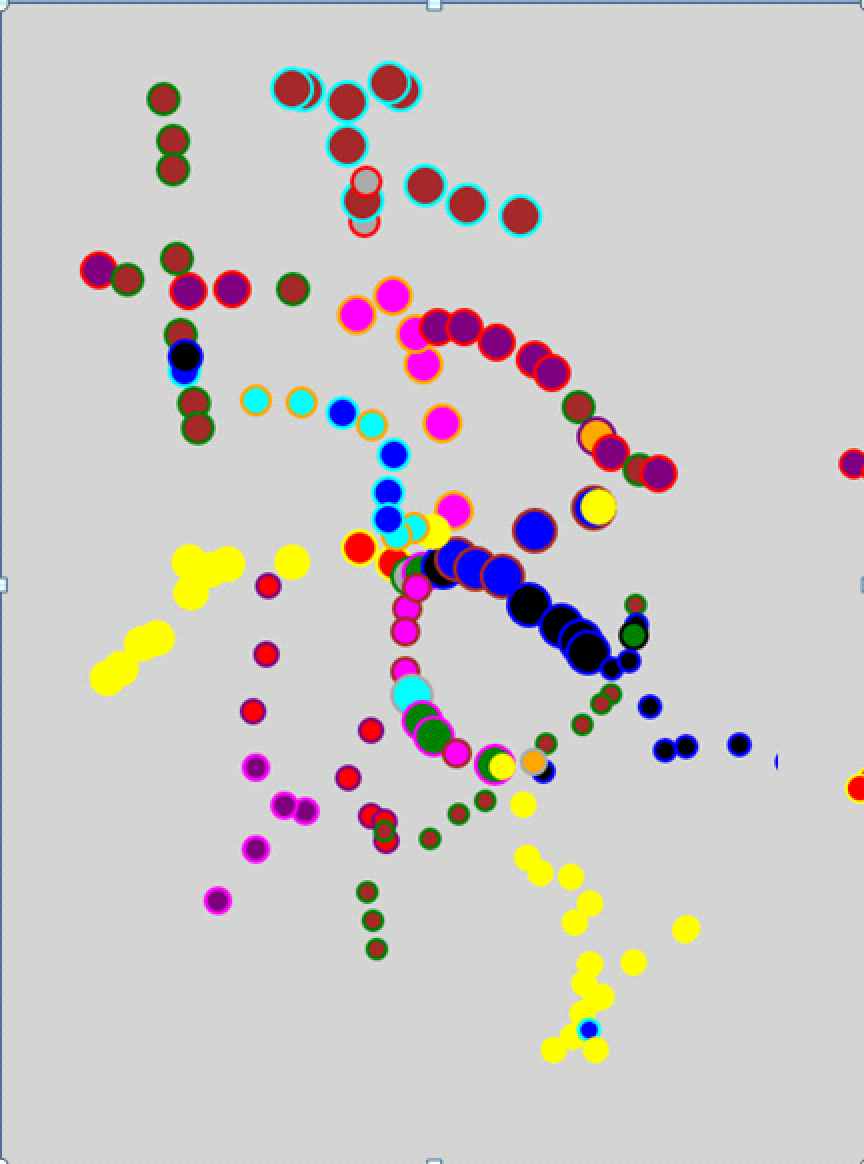
\includegraphics[width=2.2in]{picture/liuliangbianquan}
					\caption{fig1}
					\label{fenqun1}
				\end{minipage}%
				\begin{minipage}{0.5\linewidth}
					\centering
					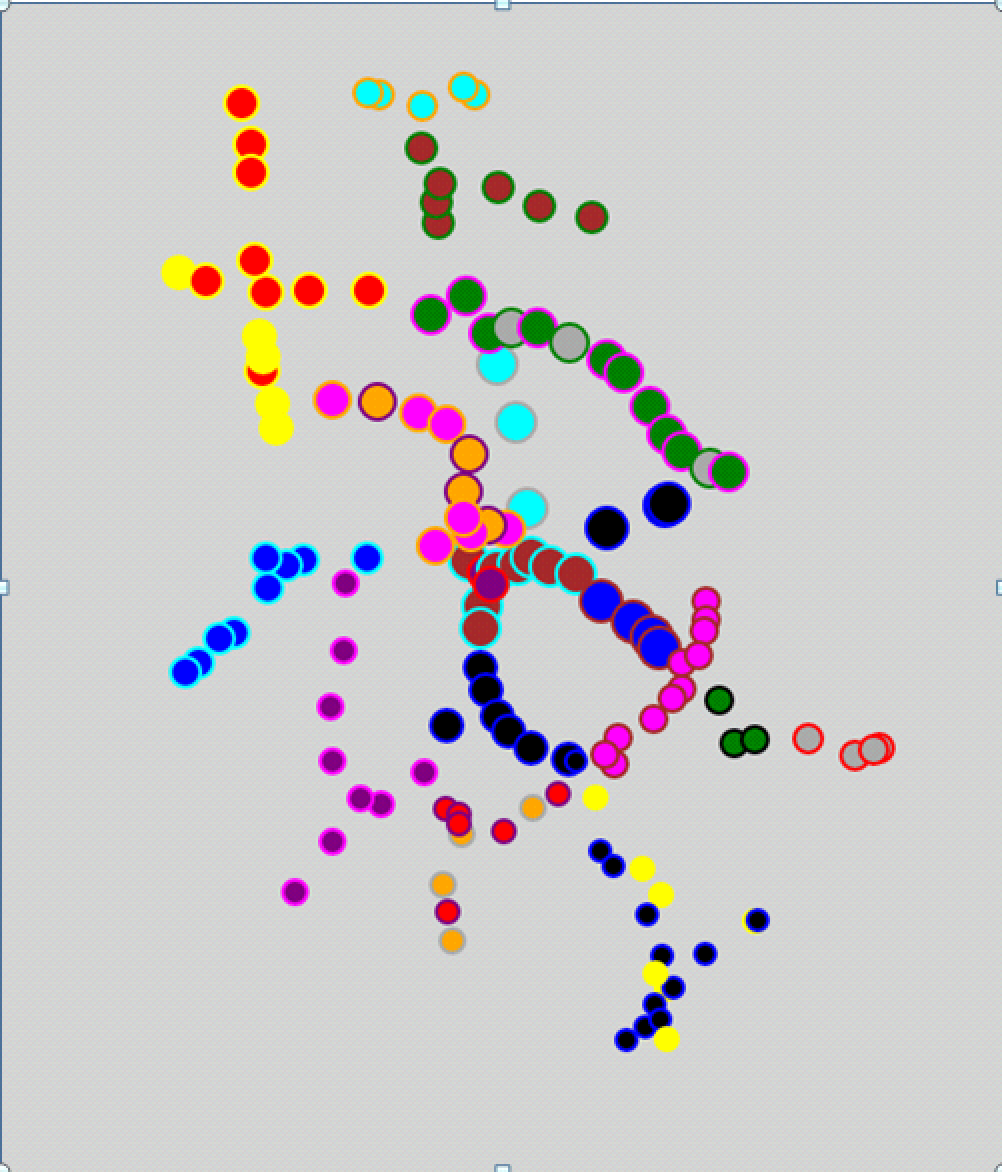
\includegraphics[width=2.2in]{picture/xiaochuguli}
					\caption{fig2}
					\label{fenqun2}
				\end{minipage}
				\end{figure}

				\begin{figure}
				\centering
				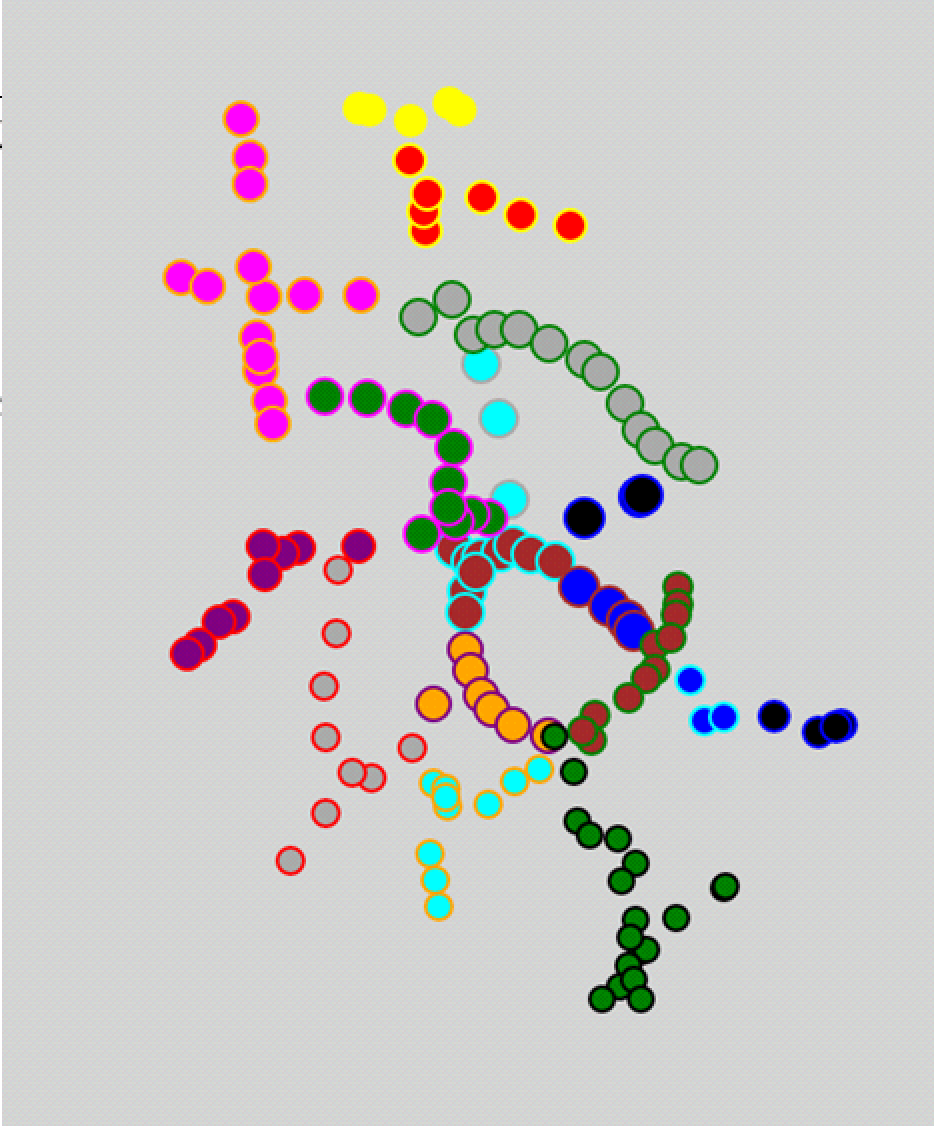
\includegraphics[width=4.4in]{picture/fenqunjieguo}
				\caption{fig1}
				\label{fenqun3}
				\end{figure}

		分群后,采用分治方法计算关键路段集合。最后将求的的关键路段带入到第一章的模型中,计算路网通行效率的提升率。图\ref{fenqunend}给出了一天时间内,基于分群算法和简单贪心方法的对比试验;图\ref{end}给出了在一周时间内两种方法的对比试验。和上一章节一样,横坐标表示时间,纵坐标表示路网通行效率的绝对值(路网通行时间)。由图可以看出,简单贪心算法和基于分群算法的关键路段挖掘算法之间的误差较为平稳,并且一直维持在一个较低的水平线上。

				\begin{figure}
				\begin{minipage}{0.5\linewidth}
					\centering
					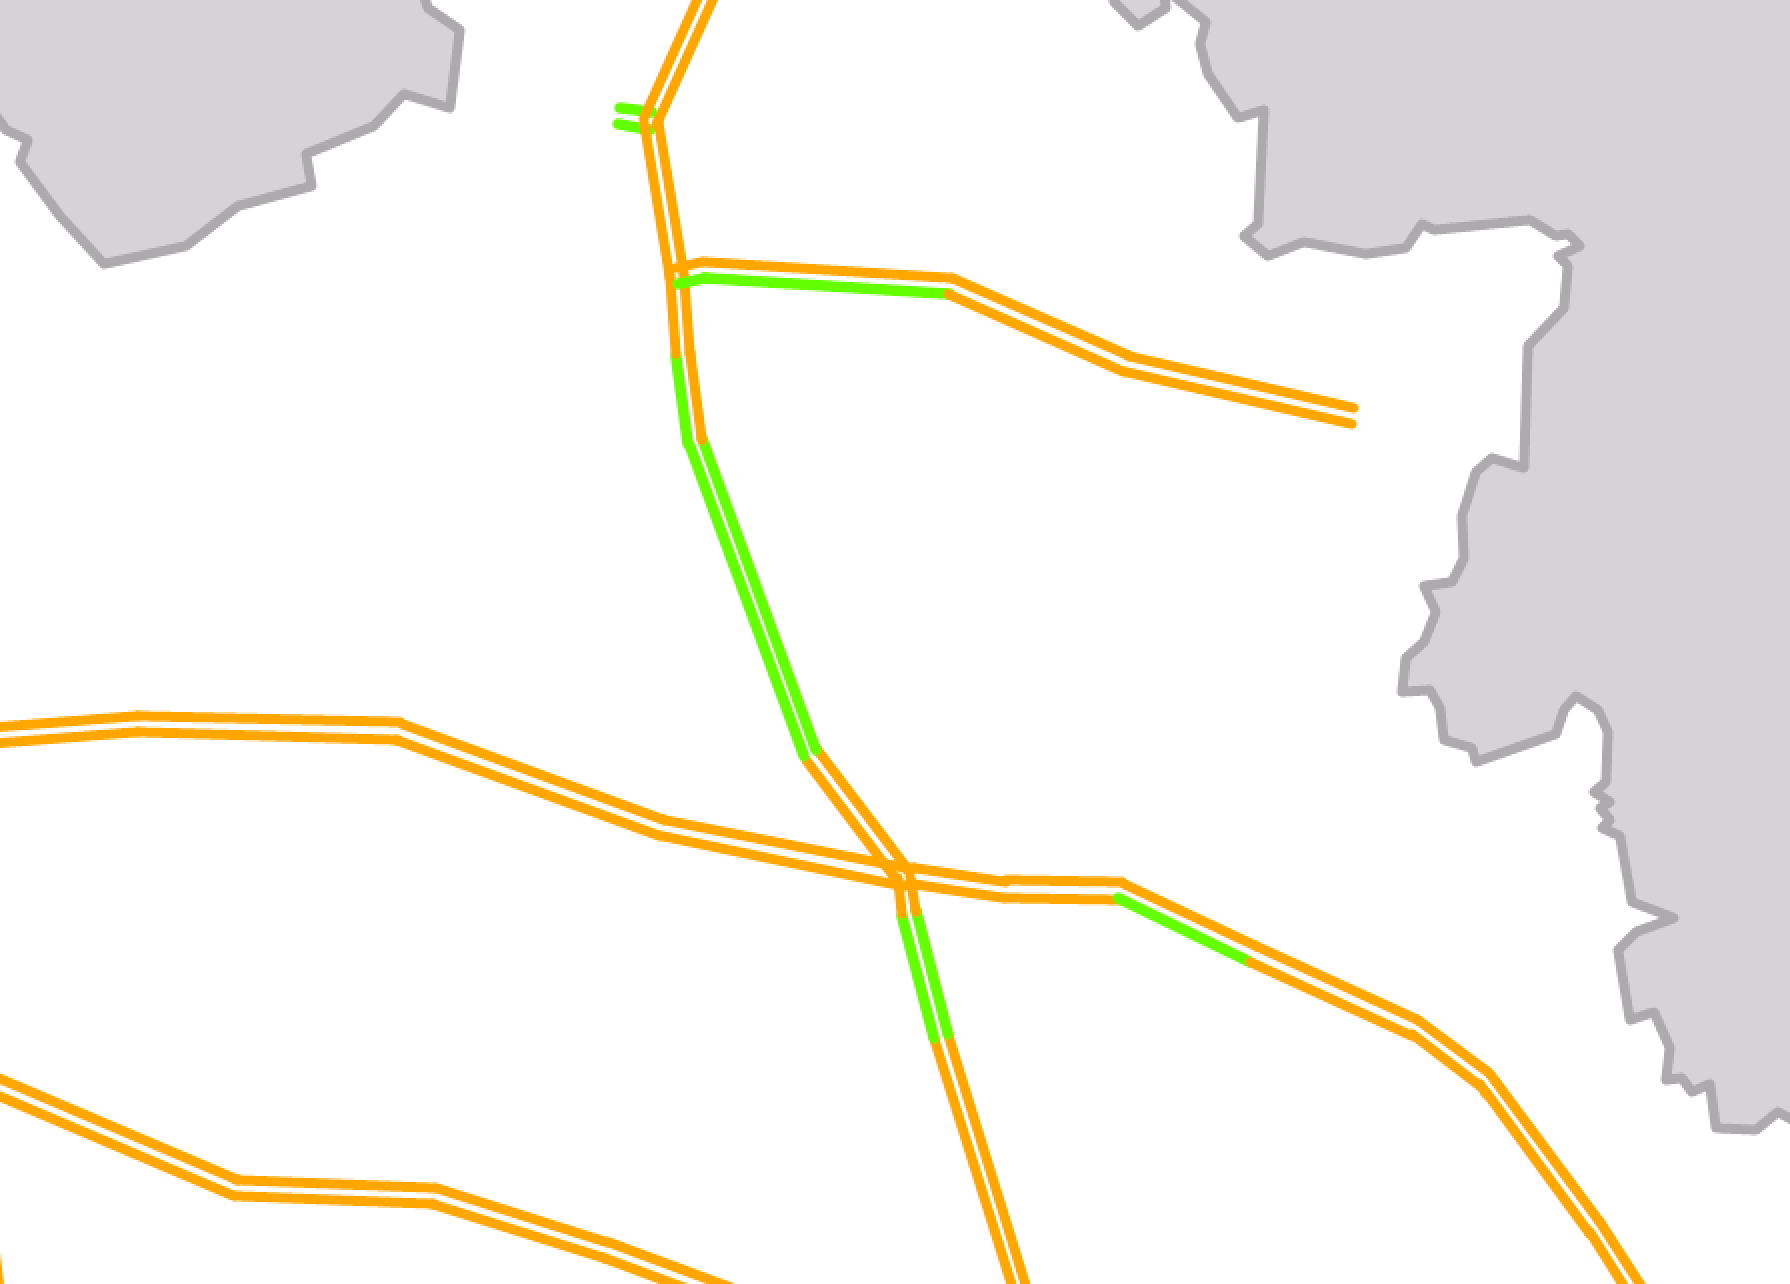
\includegraphics[width=2.2in]{picture/greedy02}
					\caption{图片还得再画}
					\label{fenqunend}
				\end{minipage}%
				\begin{minipage}{0.5\linewidth}
					\centering
					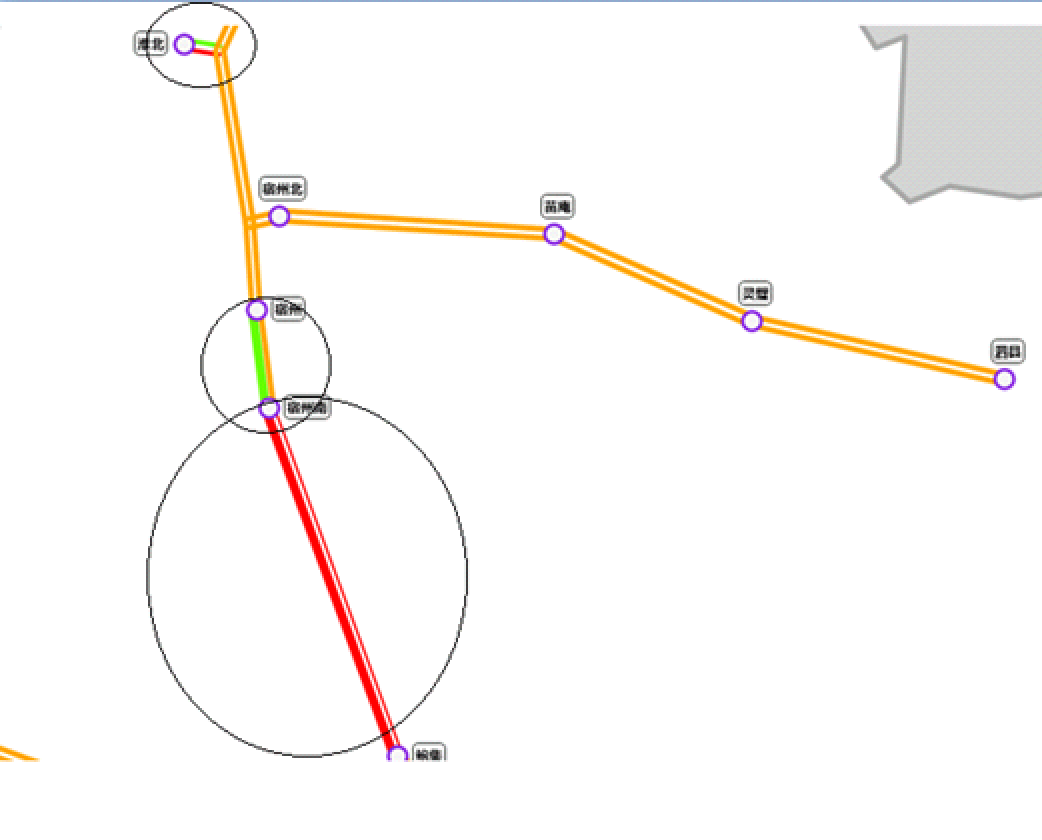
\includegraphics[width=2.2in]{picture/shequnhuafen}
					\caption{图片还得再画}
					\label{end}
				\end{minipage}
				\end{figure}

		下图给出不同方法选出的关键路段集合,图\ref{jihe1}给出了枚举方法选出的关键路段集合,图\ref{jihe2}给出了简单贪心算法给出的关键路段集合,图\ref{jihe3}给出了结合社群划分的关键节点识别算法的结果,图\ref{jihe4}给出了基于统计学的关键节点集合。观察图\ref{jihe1}和图\ref{jihe2},发现两者选取的关键节点具有很强的相似性。

				\begin{figure}
				\begin{minipage}{0.5\linewidth}
					\centering
					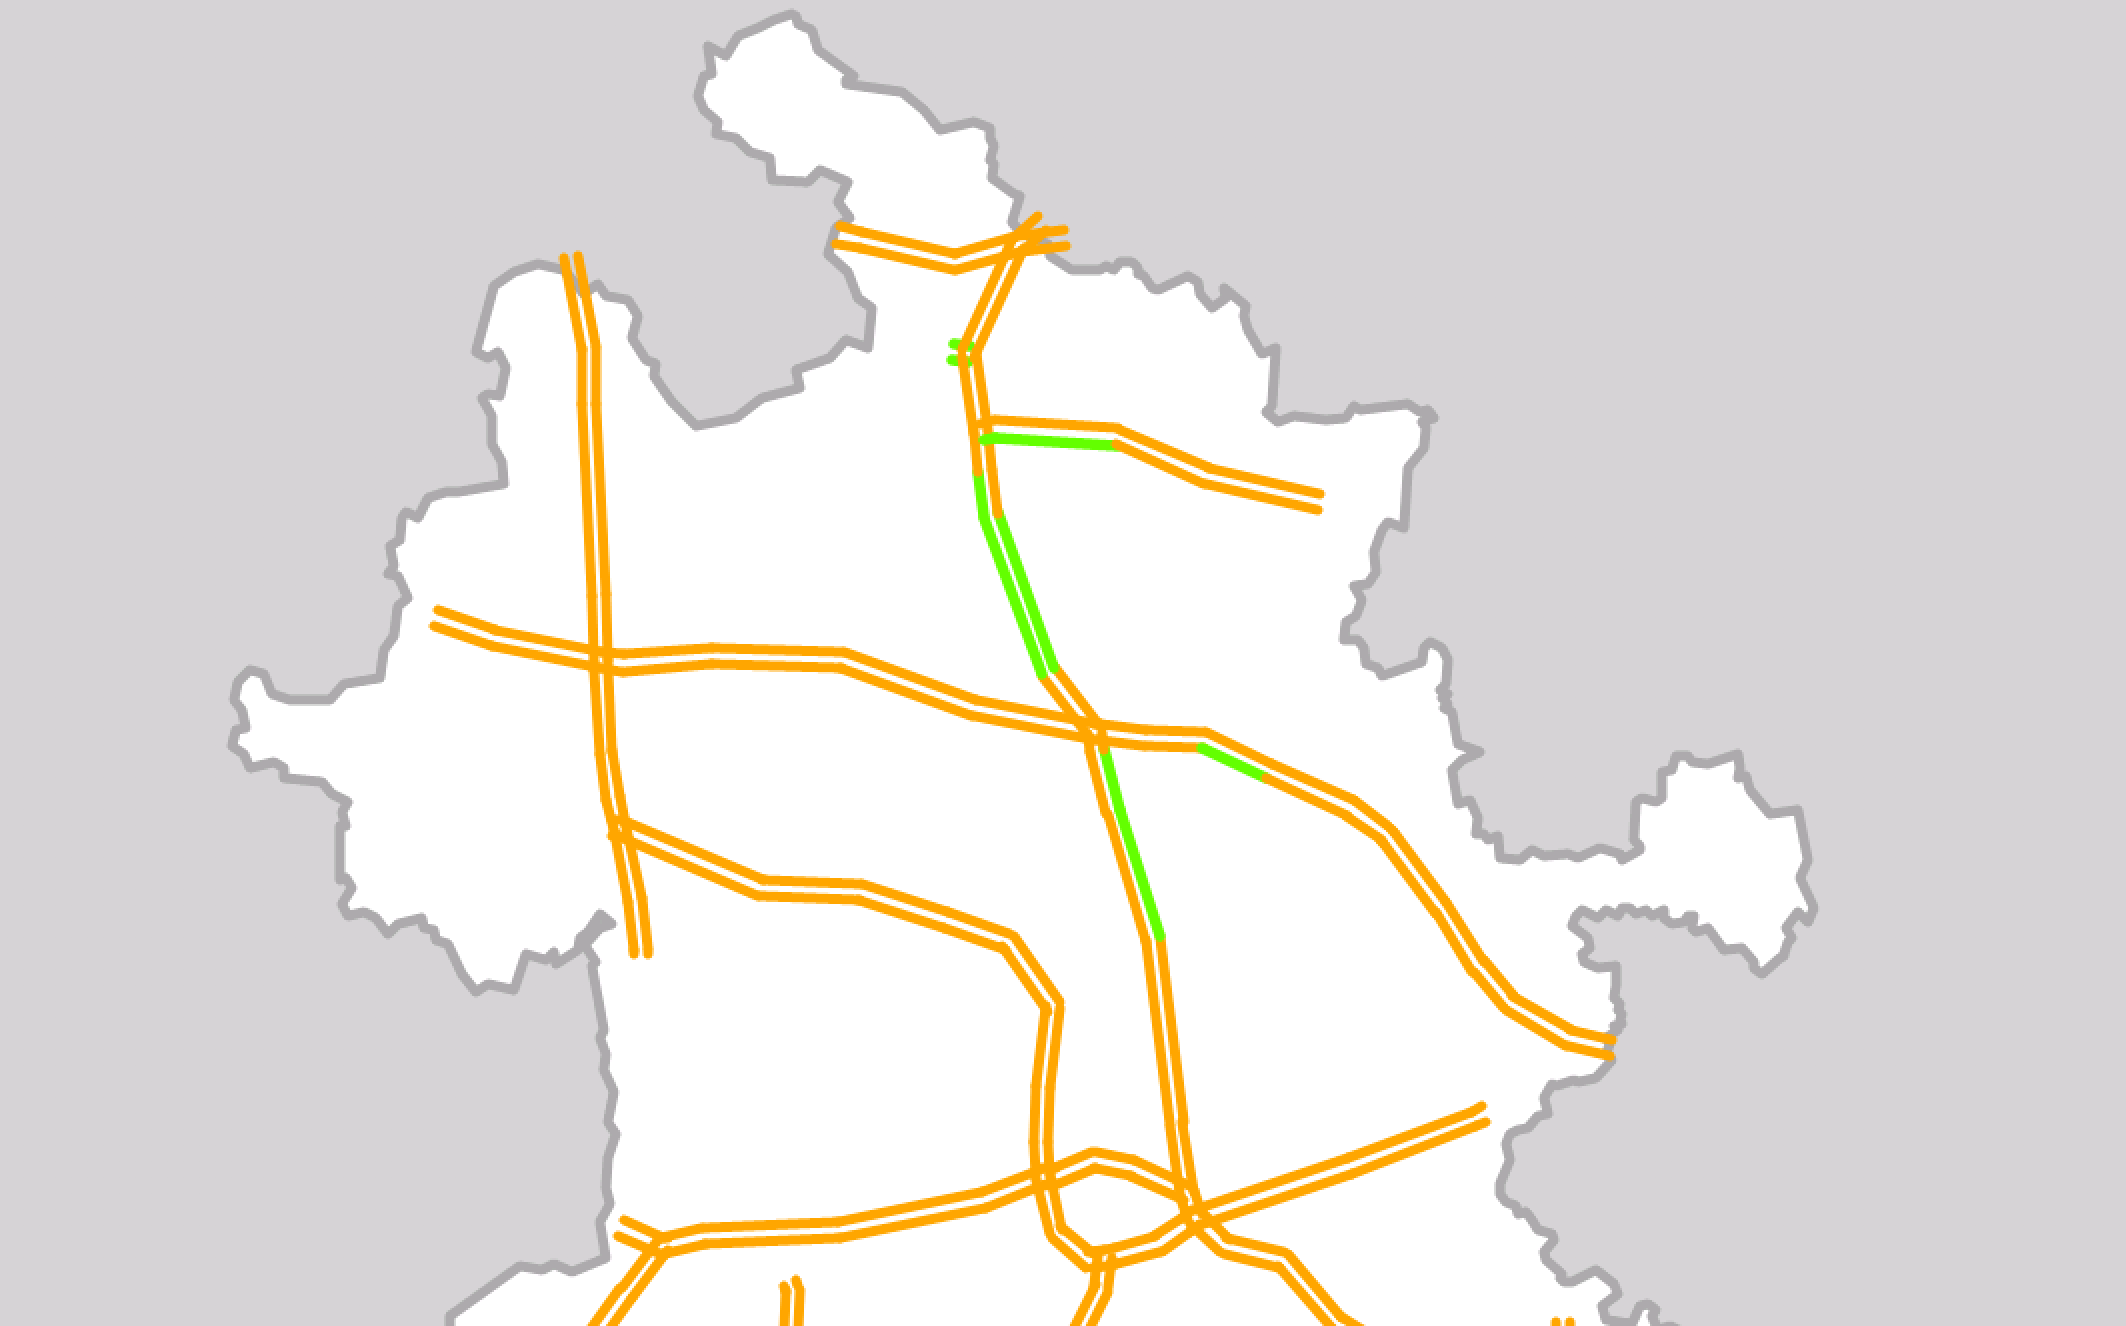
\includegraphics[width=2.2in]{picture/meiju}
					\caption{fig1}
					\label{jihe1}
				\end{minipage}%
				\begin{minipage}{0.5\linewidth}
					\centering
					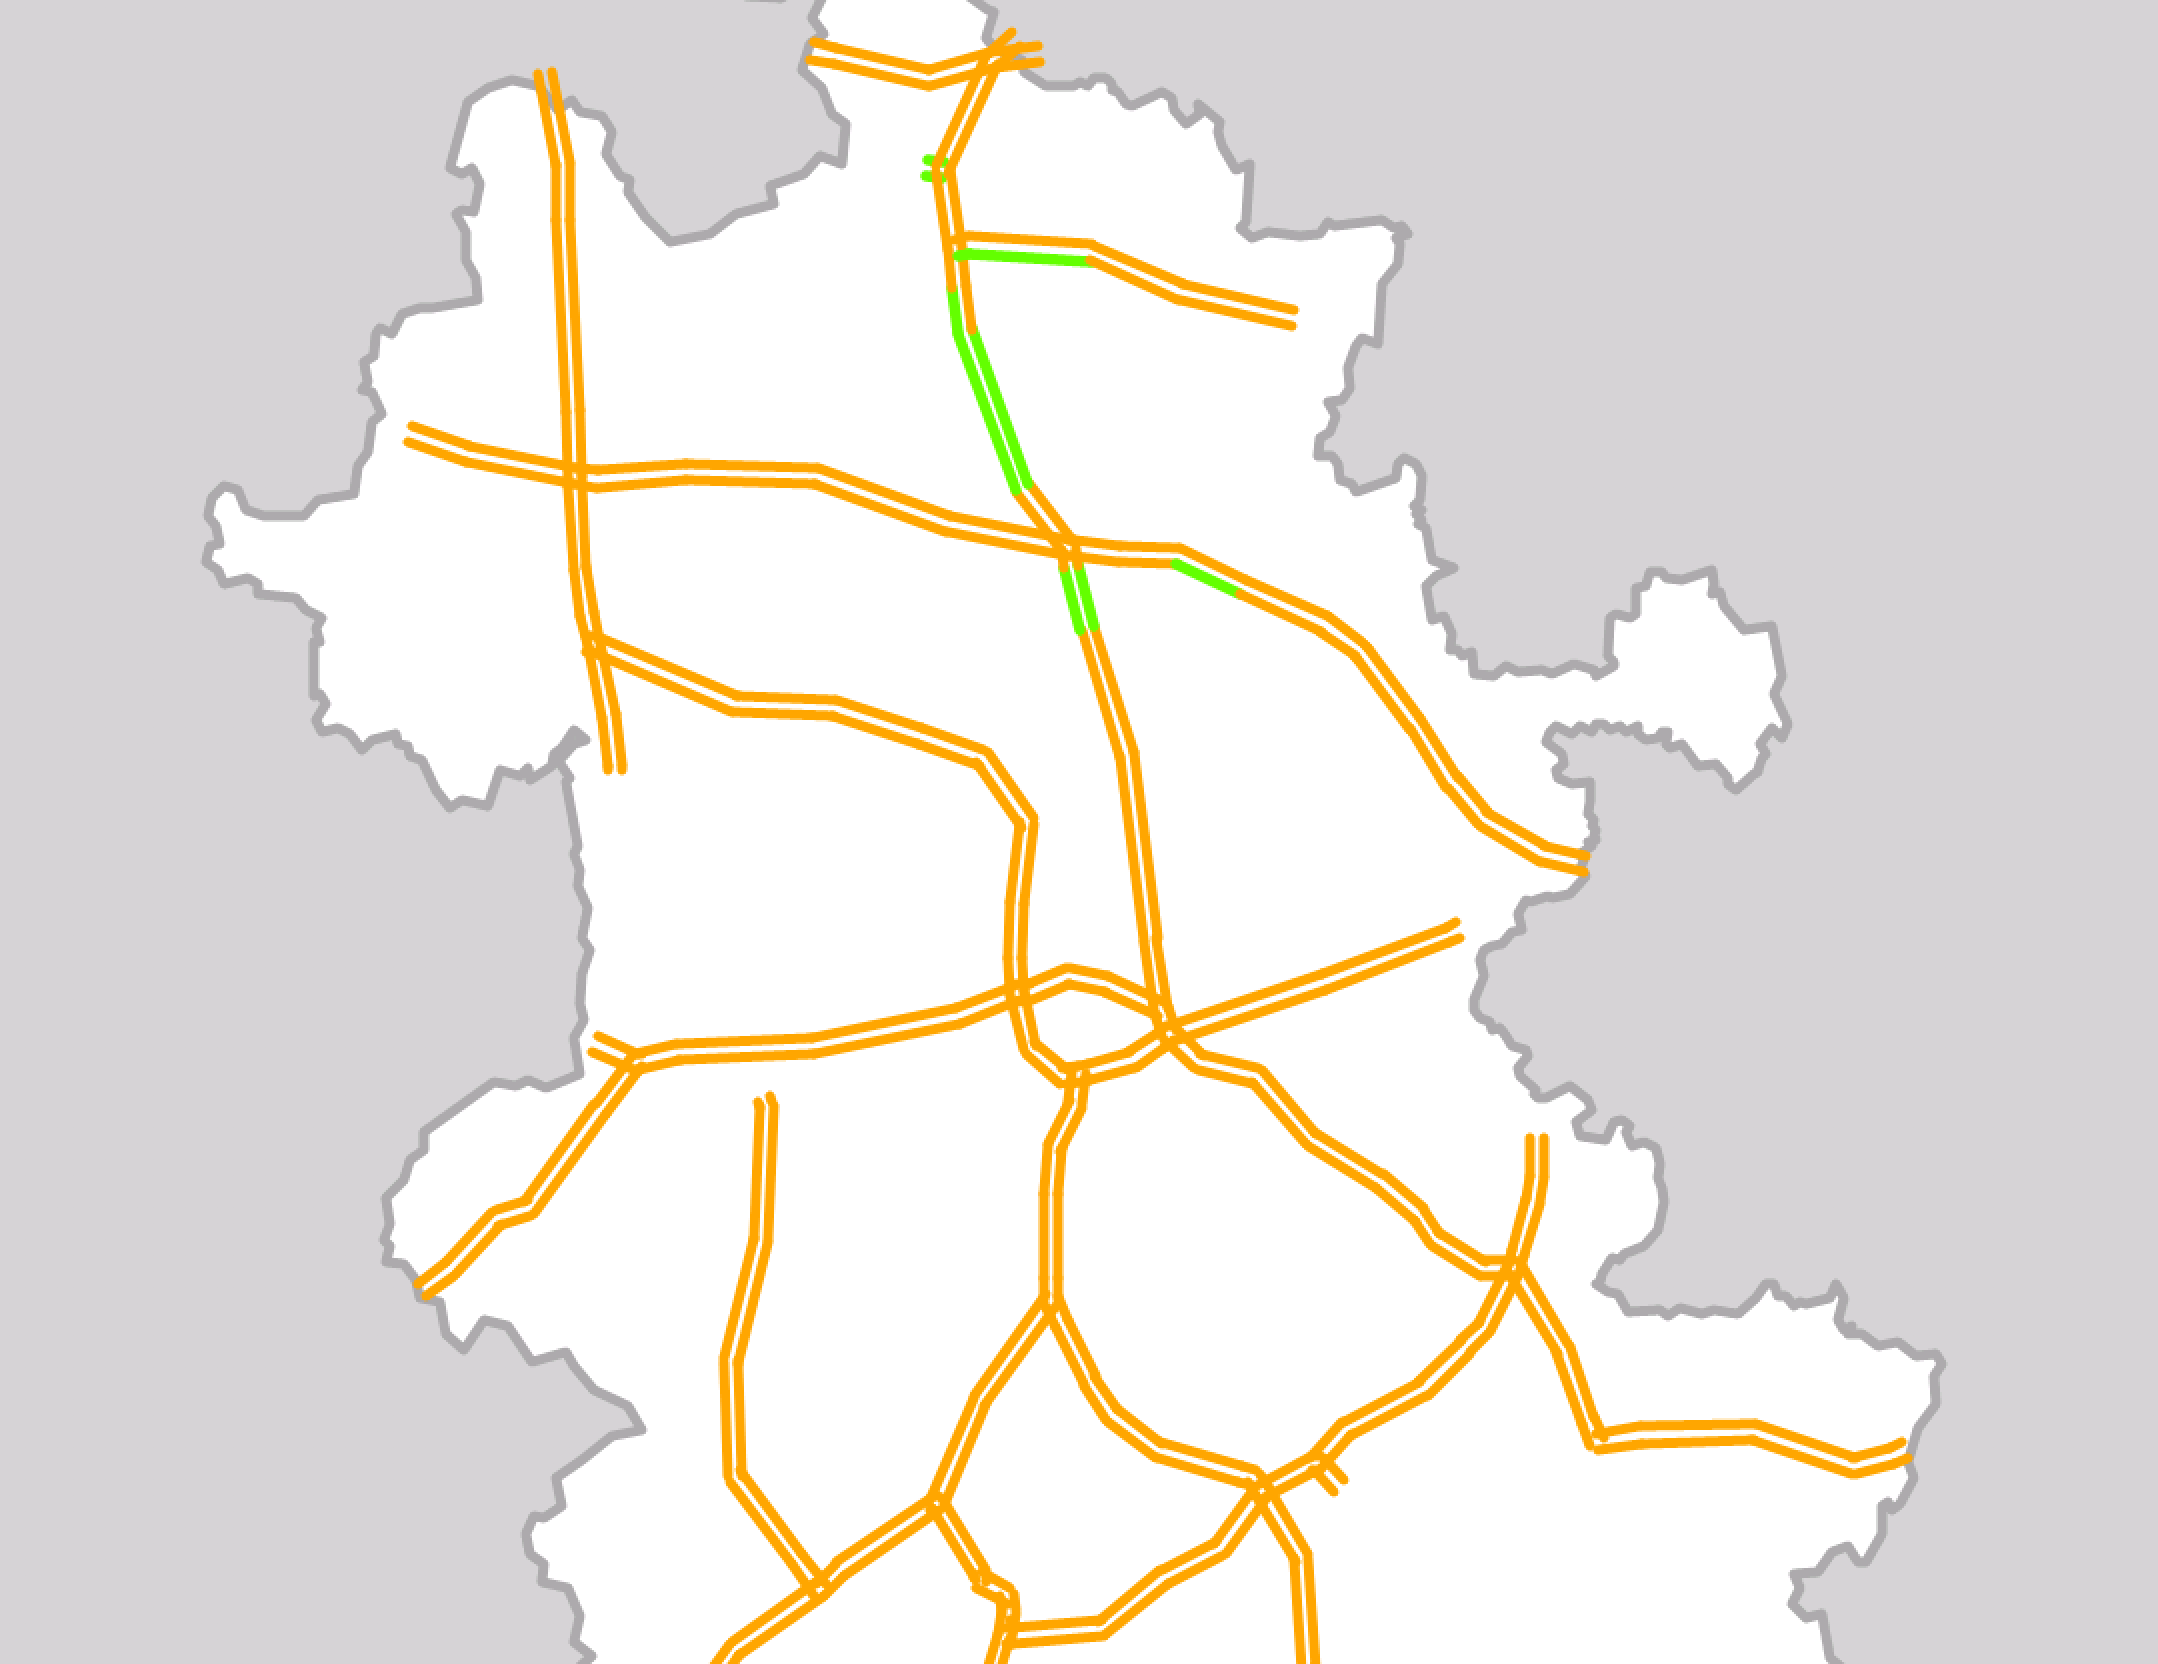
\includegraphics[width=2.2in]{picture/greedy01}
					\caption{fig2}
					\label{jihe2}
				\end{minipage}
				\end{figure}

				\begin{figure}
				\begin{minipage}{0.5\linewidth}
					\centering
					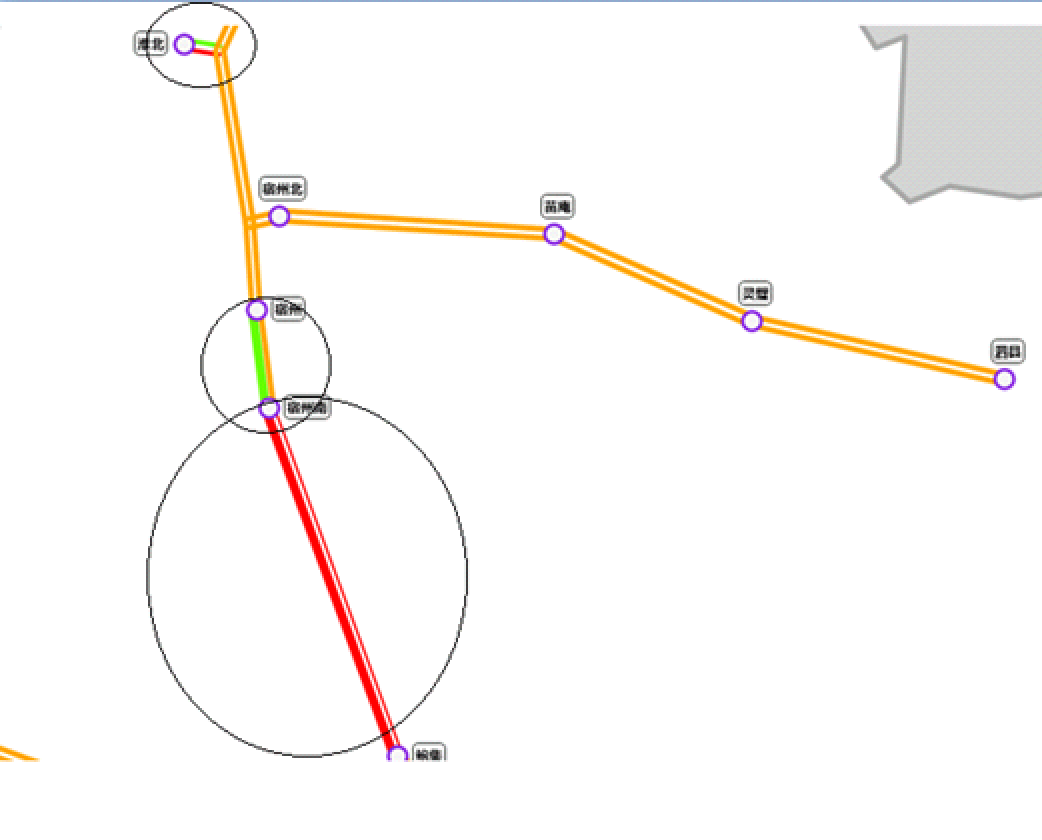
\includegraphics[width=2.2in]{picture/shequnhuafen}
					\caption{fig1}
					\label{jihe3}
				\end{minipage}%
				\begin{minipage}{0.5\linewidth}
					\centering
					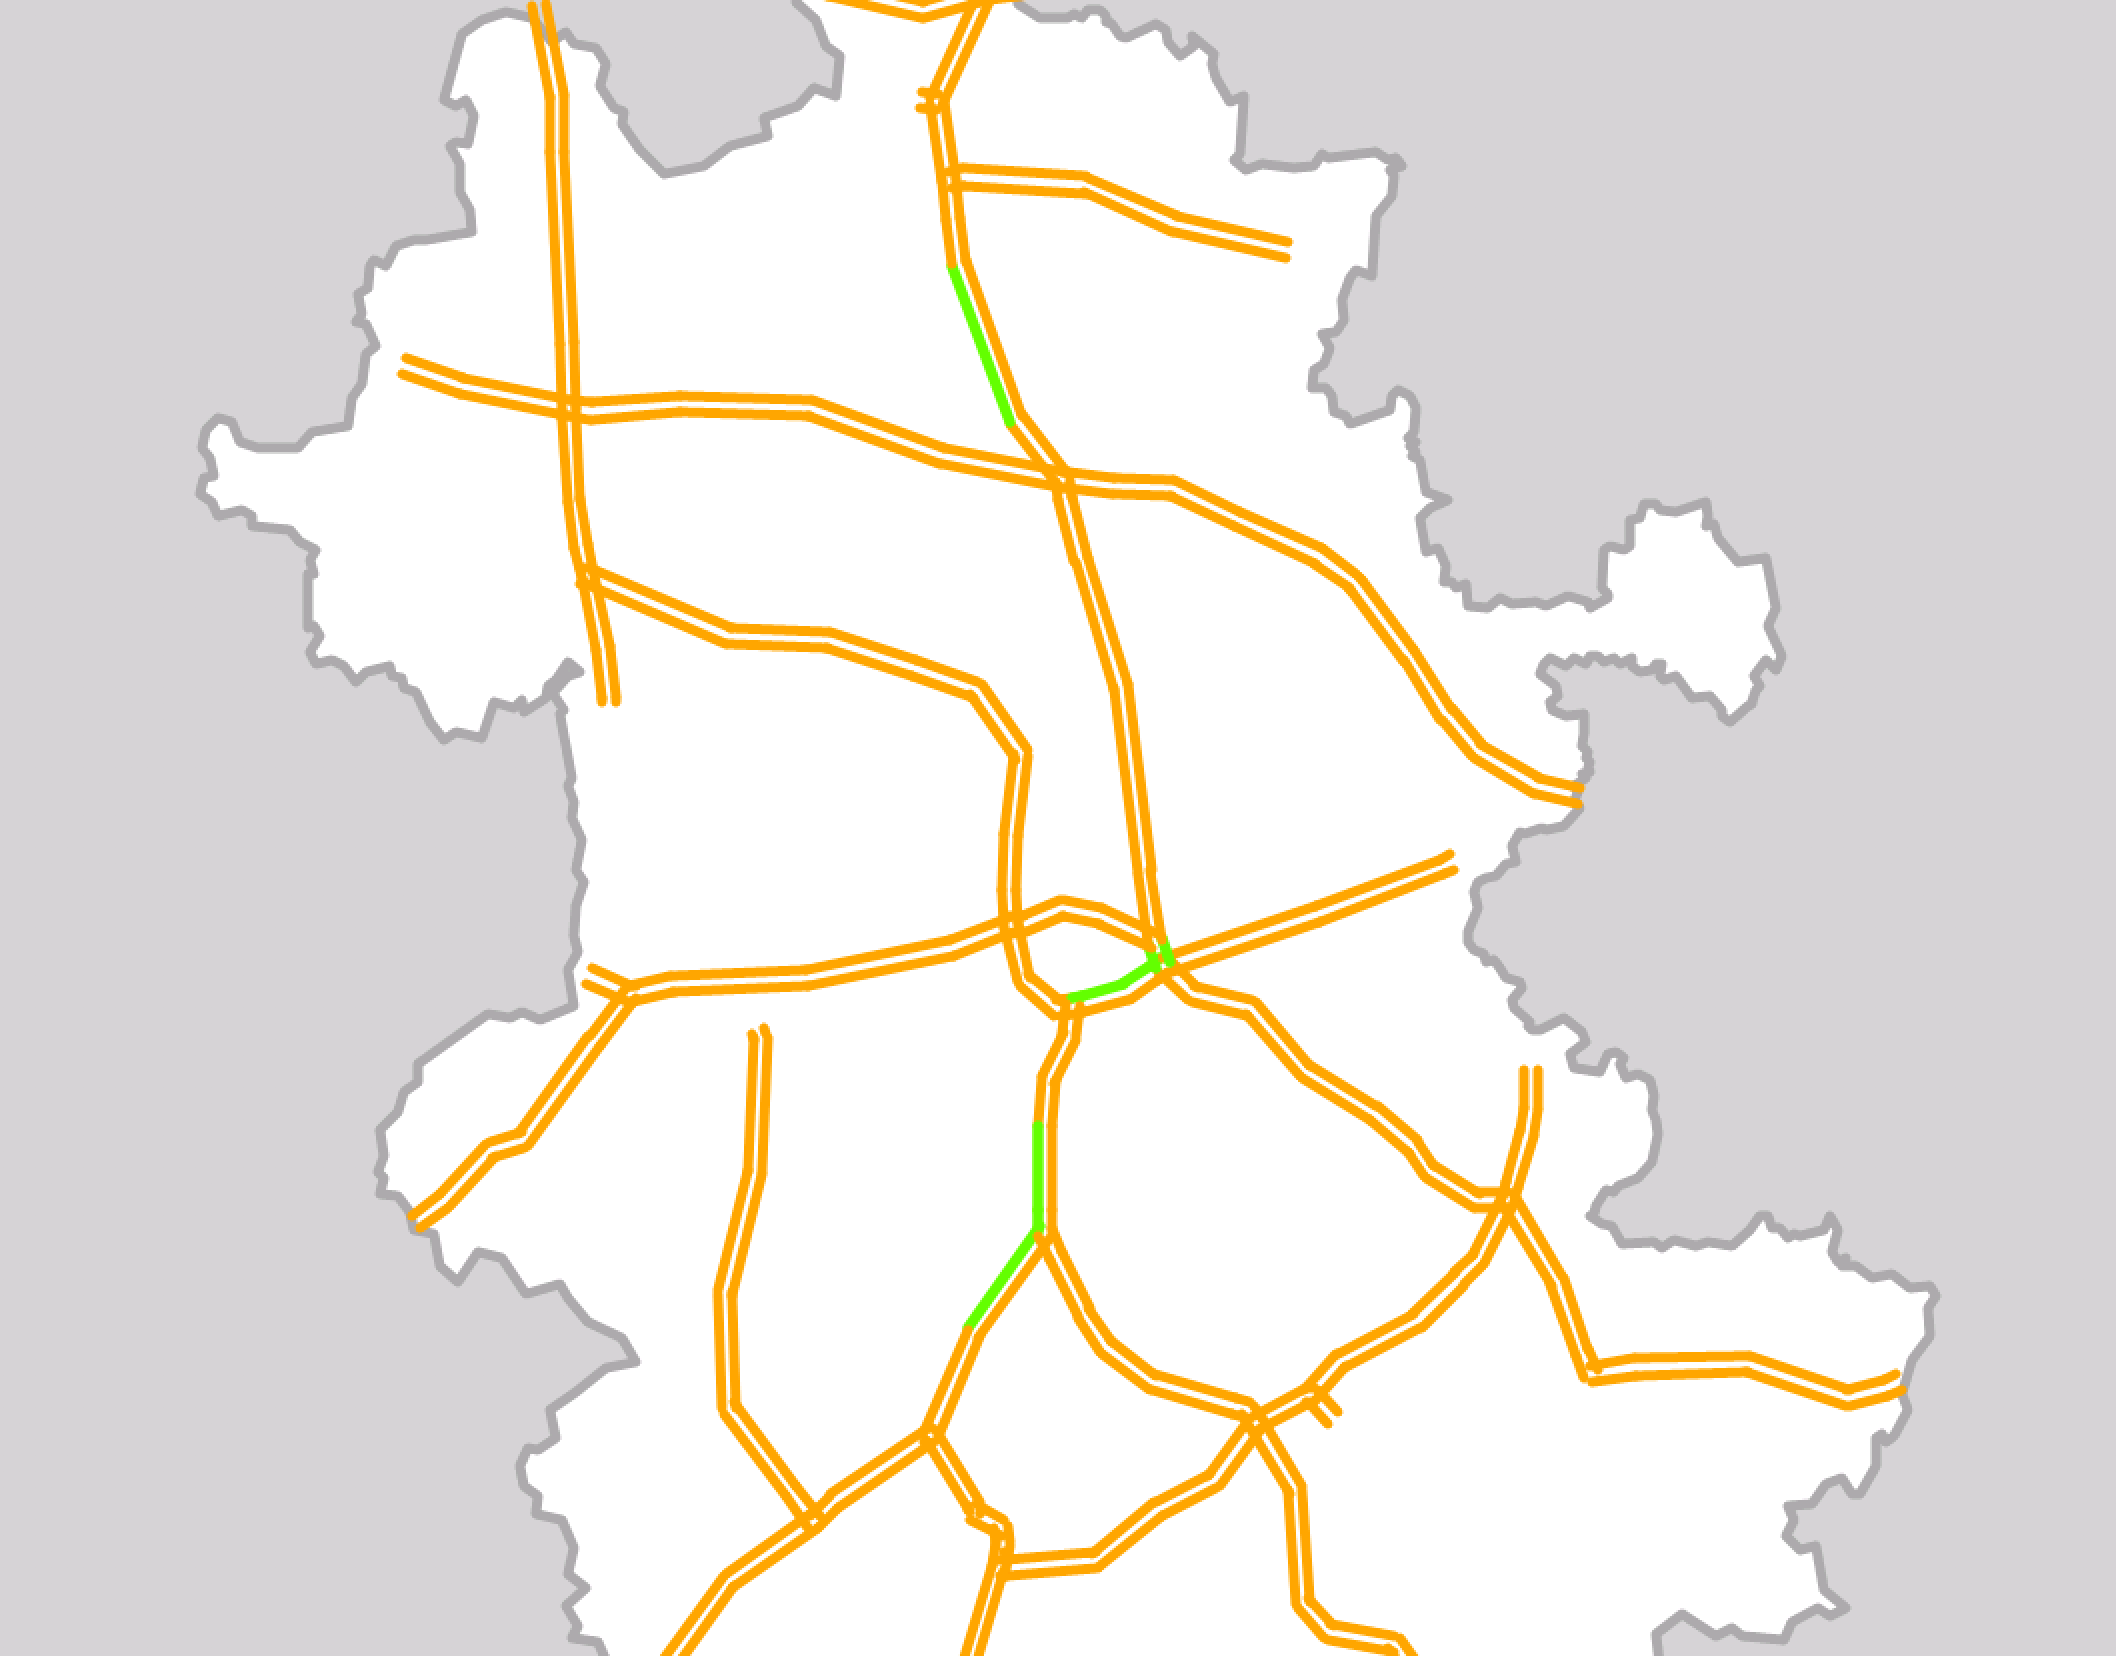
\includegraphics[width=2.2in]{picture/hotsection01}
					\caption{fig2}
					\label{jihe4}
				\end{minipage}
				\end{figure}

		误差分析:

				\begin{table}[h]
				\centering
				\begin{tabular}{|c|c|c|}
				\hline
				\hline
				  &  枚举-直接贪心 &  直接贪心-基于社群划分 \\
				\hline
				 一小时 &  14.63\% &  12.89\% \\
				\hline
				 一天 &  13.25\% &  13.26\% \\
				\hline
				 一周 &  13.10\% &  15.61\% \\
				\hline
				 一月 &  12.99\% &  11.59\% \\
				\hline
				\end{tabular}
				\caption{example of table}
				\label{table1}
				\end{table} 

		表\ref{table1}描述了枚举方法和直接贪心方法之间的误差,直接贪心和基于社群划分方法之间的误差。误差由高速路网的通行效率计算,可以看出误差在允许范围内。

		关键节点选取误差分析:

				\begin{table}[h]
				\centering
				\begin{tabular}{|c|c|c|}
				\hline
				\hline
				   &   枚举-直接贪心 &   枚举-基于社群划分 \\
				\hline
				  一小时 &   0.18\% &   0.25\% \\
				\hline
				  一天 &   0.14\% &   0.20\% \\
				\hline
				  一周 &   0.15\% &   0.19\% \\
				\hline
				  一月 &   0.14\% &   0.18\% \\
				\hline
				\end{tabular}
				\caption{example of table}
				\label{table2}
				\end{table} 

		表\ref{table2}分析了关键路段选取情况的误差,采用欧式距离来刻画区别。可以看出,随着数据集的扩大,基于社群划分方法的关键节点准确率逐步上升。

		运行效率分析:

				\begin{table}[h]
				\centering
				\begin{tabular}{|c|c|c|c|c|}
				\hline
				\hline
				   &   枚举 &   直接贪心 &   基于社群划分 &   基于统计 \\
				\hline
				  一小时 &   1day &   30min &   2min &   1min \\
				\hline
				  一天 &   6day &   2h &   5min &   2min \\
				\hline
				  一周 &  7day &   3h &   6min &   5min \\
				\hline
				  一月 &   7day &   3h &   7min &   8min \\
				\hline
				\end{tabular}
				\caption{example of table}
				\label{table3}
				\end{table} 

		由表\ref{table3}可以看出,基于社群划分方法可以将整个算法的时间复杂度再降一个数量级,而结合表\ref{table1}来看,精度误差处于可接受范围$(1/e)$。

	\section{本章小结}
		本章提出了面向高速公路的社群划分方法,首先分析了传统方法的局限性,然后结合高速公路的独有特性,采用多变权值-模拟退火结合的方法,实现符合高速公路网络特点的社群划分方法。